\documentclass{article}
\usepackage{graphicx} % Required for inserting images
\usepackage{float}
\title{Lesson 17 Homework - Proof Writing}
\author{William Wang}
\date{February 2025}

\begin{document}

\maketitle

\section{Question 1}
\begin{figure}[H]
    \centering
    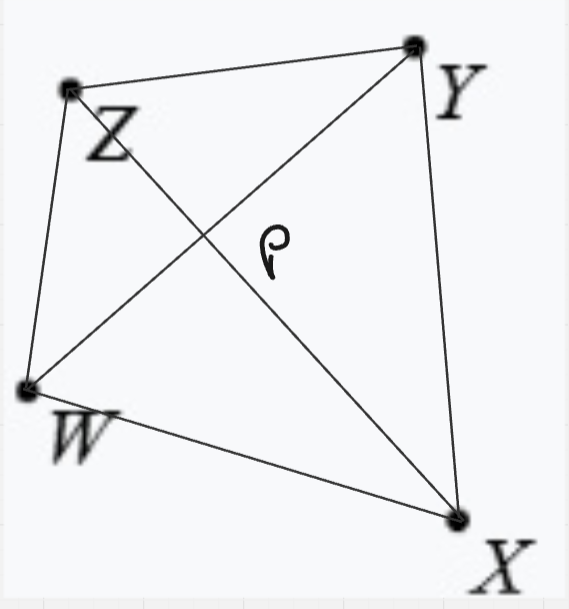
\includegraphics[width=1\linewidth]{q1.png}
\end{figure}
Let \(P\) be the point where we place the stake. We want to make \(WP+XP+YP+ZP\) as small as possible. Applying the Triangle Inequality to \(\triangle WPY\) gives \(WP+YP\ge WY\) and applying it to \(\triangle XPZ\) gives \(XP+ZP\ge XZ\). Adding these two inequalities gives \(WP+XP+YP+ZP\ge WY+XZ\). This only works if \(P\) lies on segments \(WY\) and \(XZ\). 

Therefore, \(P\) should be on the intersection between \(WY\) and \(XZ\). 

\section{Question 2}
\begin{figure}[H]
    \centering
    
\includegraphics[width=1\linewidth]{q2.png}
\end{figure}
Since in a convex quadrilateral, the diagonals intersect inside the quadrilateral, we know that diagonals form triangles. 

We can use the triangle inequality for \(\triangle ABX\) to get \(AX + XB > AB\) and \(\triangle DXC\) to get \(DX + CX = DC\) and \(\triangle AXD\) to get \(AX + XD > AD\) and \(\triangle BXC\) to get \(BX + CX> BC\). 

By combining all these inequalities, we get 
\[2AX + 2BX + 2CX + 2DX > AB + BC + CD + AD\]
which simplifies down to 
\[2AC + 2BC > AB + BC + CD + AD\]
\[AC + BC > \frac{AB + BC+CD+AD}{2}\]
Therefore, the sum of the diagonals in a convex quadrilateral is greater than the semi perimeter. 
\end{document}
